\documentclass[10pt,twocolumn]{article}

\usepackage[a4paper,margin=17mm,columnsep=6mm]{geometry}
\usepackage{times}
\usepackage{microtype}
\usepackage{graphicx}
\usepackage{booktabs}
\usepackage{multirow}
\usepackage{amsmath,amssymb}
\usepackage{xcolor}
\usepackage{url}
\usepackage{hyperref}
\usepackage{enumitem}
\usepackage{caption}

\definecolor{adapterblue}{HTML}{2563EB}
\definecolor{softblue}{HTML}{EAF2FF}
\definecolor{softorange}{HTML}{FFF1E8}
\definecolor{softgreen}{HTML}{EAF8EF}
\hypersetup{
  colorlinks=true,
  linkcolor=adapterblue,
  citecolor=adapterblue,
  urlcolor=adapterblue,
  pdftitle={Timing Before Talking: Time Adapters for Low-Latency Turn-Taking in Spoken Language Models},
  pdfauthor={Towa Yoshida}
}
\setlist{nosep,leftmargin=*}
\captionsetup{font=small,labelfont=bf}
\setlength{\parindent}{1em}
\setlength{\parskip}{0pt}
\newcommand{\model}{Qwen2.5-Omni-3B}
\newcommand{\adapter}{Time Adapter}
\newcommand{\code}[1]{\texttt{#1}}

\title{\vspace{-1.4em}\textbf{Timing Before Talking: Time Adapters for Low-Latency\\Turn-Taking in Spoken Language Models}}
\author{Towa Yoshida\\
Rissho University, Tokyo, Japan\\
\href{mailto:onigirikiller@proton.me}{onigirikiller@proton.me}\quad
\href{https://orcid.org/0009-0002-1715-0219}{ORCID: 0009-0002-1715-0219}}
\date{Research Preprint --- July 2026}

\begin{document}
\maketitle

\begin{abstract}
Spoken language models can produce fluent responses, but deciding \emph{when} to speak remains a separate systems problem. Running full generation at every audio tick is expensive, while a model that ignores elapsed silence may interrupt, respond late, or miss opportunities for a short backchannel. We study a compact \adapter{} that maps explicit streaming-time features to a residual injected into an audio-language model hidden layer. A high-frequency decision path scores three single-token actions---wait (\code{/W}), backchannel (\code{/B}), and support/respond (\code{/S})---and invokes text or speech generation only when needed. On a generated sequential benchmark of 600 utterances evaluated at ten silence durations, a proxy decision head reaches 0.989 macro F1. However, feeding the same residual to the frozen base language-model head reaches only 0.428 macro F1, revealing an objective-alignment failure rather than a lack of temporal information. Training the action-token logits directly with low-rank adaptation raises macro F1 to 0.998 in an audio-only setting; a control-token-plus-short-response objective also reaches 0.998. In a four-case local pseudo-realtime check on an RTX 4090, action scoring has 309.1 ms p95 latency and 99.3\% of 137 ticks complete within 500 ms, excluding asynchronous response generation. These results are engineering evidence from synthetic and templated evaluation, not an independent natural-dialogue benchmark. We release source code, ablations, and this paper to make both the positive and negative findings reproducible.
\end{abstract}

\section{Introduction}

Turn-taking is a continuous prediction problem: a dialogue system must distinguish a completed turn from a hesitation, self-repair, requested pause, or point where a minimal acknowledgment is appropriate. Prior work models turn transitions from lexical, prosodic, or voice-activity signals \cite{skantze2017continuous,ekstedt2020turngpt,ekstedt2022vap,leishman2026lexical}. Modern speech--language models improve response content and audio generation, yet strong language modeling does not automatically provide calibrated timing behavior \cite{umair2024when}. Full-duplex systems such as Moshi demonstrate that low-latency speech interaction is possible, but tightly integrated training is costly \cite{defossez2024moshi}.

This work asks a narrower, practical question: \emph{can a small external representation of streaming time steer a pretrained audio-language model without requiring full generation at every tick?} We explore a residual adapter attached to the Thinker component of \model{} \cite{xu2025qwenomni}. The adapter encodes elapsed silence and related streaming state. A compact decision path emits one of three actions, allowing expensive response generation to remain event-driven.

The study is deliberately diagnostic. A high-performing auxiliary classifier does not prove that the model's native output head can use the same residual. We therefore trace the design through three stages: (1) a proxy decision head, (2) frozen base language-model logits under hidden-state injection, and (3) directly trained single-token logits using LoRA \cite{hu2021lora}. The failed middle stage is central to the result.

Our contributions are:
\begin{itemize}
  \item a small temporal residual interface for streaming audio-language models;
  \item controlled ablations that separate correct timing from zero, shuffled, random, and non-time numeric vectors;
  \item evidence that representation quality and output-objective alignment are distinct requirements; and
  \item a label-first runtime in which frequent action scoring is separated from asynchronous response generation.
\end{itemize}

\begin{figure*}[t]
\centering
\setlength{\fboxsep}{8pt}
\colorbox{softblue}{\parbox{0.18\textwidth}{\centering\textbf{Audio prefix}\\waveform + dialogue prompt}}
\hfill$\longrightarrow$\hfill
\colorbox{softblue}{\parbox{0.18\textwidth}{\centering\textbf{Audio LM}\\hidden state $h_{\ell}$}}
\hfill$+$\hfill
\colorbox{softorange}{\parbox{0.19\textwidth}{\centering\textbf{Time Adapter}\\$z_t\mapsto a_t$}}
\hfill$\longrightarrow$\hfill
\colorbox{softgreen}{\parbox{0.21\textwidth}{\centering\textbf{Action token}\\\code{/W}: silence\quad \code{/B},\code{/S}: generate}}
\caption{Proposed label-first architecture. The high-frequency path computes a temporal residual and scores only three action tokens. Text and speech generation are triggered asynchronously for \code{/B} or \code{/S}; they are not part of every timing tick.}
\label{fig:architecture}
\end{figure*}

\section{Related Work}

\paragraph{Turn-transition prediction.}
Continuous turn-taking models estimate future speech activity or transition relevance from acoustic and lexical context \cite{skantze2017continuous,ekstedt2022vap}. TurnGPT represents turn completion as a language-modeling problem and shows that text carries useful transition information \cite{ekstedt2020turngpt}. Recent analysis explicitly separates temporal from lexical predictability \cite{leishman2026lexical}. Our approach does not replace these predictors; it tests an interface for injecting externally measured streaming time into a general audio-language model.

\paragraph{Spoken foundation models.}
End-to-end speech systems increasingly interleave listening and speaking. Moshi uses a streaming, multi-stream architecture for real-time dialogue \cite{defossez2024moshi}. Qwen2.5-Omni jointly processes text, images, audio, and video and generates speech through separate Thinker and Talker components \cite{xu2025qwenomni}. We use its 3B research model as a testbed and keep the fast decision path in the Thinker. The goal is an adapter-style intervention rather than pretraining a duplex foundation model.

\paragraph{Parameter-efficient alignment.}
LoRA learns low-rank updates while freezing the base model \cite{hu2021lora}. Here it serves a specific purpose: aligning the native next-token logits with timing actions after a frozen-head experiment exposes an objective mismatch. This is not merely a parameter-efficiency comparison.

\section{Method}

\subsection{Temporal state and residual injection}

At streaming step $t$, the controller constructs
\begin{equation}
z_t=[s_t,\Delta t_t,u_t,q_t,c_t],
\end{equation}
where $s_t$ is elapsed silence, $\Delta t_t$ is the interval since the previous decision tick, $u_t$ is elapsed utterance time, $q_t$ indicates whether the user is speaking, and $c_t$ indicates whether the ASR hypothesis changed. The implementation applies a logarithm to elapsed silence before normalization. A small multilayer perceptron $A_{\phi}$ outputs a residual $a_t=A_{\phi}(z_t)$ with the model hidden width.

Let $h_{\ell,i}$ be hidden state $i$ at layer $\ell$. The main configuration injects the residual at layer 3 for every token position:
\begin{equation}
h'_{\ell,i}=h_{\ell,i}+\alpha a_t,\qquad \alpha=4.
\label{eq:inject}
\end{equation}
The adapter is first trained to reconstruct the difference between hidden states produced with and without an explicit textual time cue. If $h^{\mathrm{exp}}$ and $h^{\mathrm{base}}$ are pooled representations, the target is $d_t=h^{\mathrm{exp}}_t-h^{\mathrm{base}}_t$ and the loss is
\begin{equation}
\mathcal{L}_{\mathrm{adapter}}=\lVert A_{\phi}(z_t)-d_t\rVert_2^2.
\end{equation}
This distills an experimentally accessible explicit-time direction; it does not claim that silence is inferred from audio alone.

\subsection{Three output objectives}

\textbf{Proxy head.} A two-layer classifier consumes the concatenation of the audio context representation and adapter residual. It predicts WAIT, BACKCHANNEL, or SUPPORT. This tests whether the representation is useful under a dedicated objective.

\textbf{Frozen LM head.} The adapter residual is injected into the generation path, but the base language-model head remains unmodified. Candidate action strings are scored from next-token logits. This tests whether hidden reconstruction alone changes the pretrained output distribution in the desired way.

\textbf{Direct action-token LoRA.} We choose single-token controls \code{/W}, \code{/B}, and \code{/S} and train their next-token logits. Rank-8 LoRA modules with scaling 16 and dropout 0.05 are applied to attention and MLP projections. The principal audio-only run uses learning rate $2\times10^{-4}$. A subsequent control-plus-response run starts from the action model, trains for two epochs at $10^{-4}$, weights the first control token by 4, and also trains a short templated response and EOS. The base model remains frozen.

\subsection{Runtime decomposition}

Figure~\ref{fig:architecture} separates two latency budgets. Every 500 ms tick updates voice activity and temporal state, evaluates the audio prefix, injects $a_t$, and scores three action logits. A \code{/W} decision ends the tick. A transition to \code{/B} or \code{/S} launches response text and speech generation outside the tick loop. This architecture cannot make generation itself free; it prevents generation from being the repeated high-frequency operation.

\section{Experimental Design}

\subsection{Generated sequential benchmark}

We generate 600 English utterance fragments with Qwen3-TTS-0.6B \cite{hu2026qwen3tts}. Each trimmed waveform is extended with zero-valued PCM at ten silence durations: 0, 0.25, 0.5, 0.75, 1, 1.5, 2, 3, 4, and 6 s. The resulting 6,000 audio timepoints are divided by utterance, not by timepoint: 500 utterances (5,000 points) for training, 50 (500 points) for validation, and 50 (500 points) for testing. Fragment overlap across splits is zero.

The label policy spans completed statements, direct questions, requested waits, self-repairs, and incomplete or vulnerable fragments. All three labels occur at every timepoint across the dataset, preventing time alone from solving the task. Labels are programmatic and therefore internally consistent, but they do not capture the ambiguity of human turn-taking annotations.

For data-scaling tests, nested training subsets contain 300, 1,000, 3,000, and 5,000 timepoints. A separate held-out-duration test removes 0.75 s and 3.0 s from train and validation. The DirectLM comparison uses the same generated family with balanced sampling; its largest audio-only result is measured on 1,000 held-out timepoints. The control-plus-response experiment uses 3,000 balanced training points and 500 points each for validation and test.

\subsection{Ablations and metrics}

We evaluate: no time residual; a zero vector; the correct adapter output; a within-context shuffled output; a random direction matched to the correct residual norm; a vector computed from non-time numeric features; and an oracle difference derived from explicit time. Accuracy and macro F1 measure individual decisions. Exact sequence accuracy requires all ten decisions for an utterance to match. The held-out-duration test probes interpolation rather than new dialogue content.

The pseudo-realtime check contains four short cases (two local recordings and two TTS examples), 137 ticks total, on one RTX 4090. Its latency distribution is a local systems measurement, not a hardware-independent benchmark.

\section{Results}

\subsection{A proxy head can exploit the residual}

Table~\ref{tab:scale} shows monotonic gains as the generated training set grows. At 5,000 training timepoints, correct-time injection reaches 0.989 macro F1 and 0.920 exact sequence accuracy. The adapter reconstruction obtains $R^2=0.986$, Pearson $r=0.993$, mean cosine similarity 0.924, and MSE 0.002 (0.148 of a zero-prediction baseline). These statistics show that the explicit-time hidden difference is predictable from the streaming features.

\begin{table}[t]
\centering
\caption{Proxy-head scaling on held-out utterances. Each utterance contributes ten timepoints.}
\label{tab:scale}
\small
\begin{tabular}{lrrrr}
\toprule
Train & Layer & Acc. & Macro F1 & Exact seq.\\
\midrule
300   & 12 & .750 & .693 & .300\\
1,000 & 3  & .930 & .924 & .650\\
3,000 & 8  & .978 & .976 & .900\\
5,000 & 8  & \textbf{.990} & \textbf{.989} & \textbf{.920}\\
\bottomrule
\end{tabular}
\end{table}

The full ablation in Figure~\ref{fig:ablation} is more informative than the headline score. No-time hidden states are already strong (0.951 macro F1), plausibly because appended silence changes the audio prefix. Correct timing adds 0.038 absolute F1, while shuffled timing falls to 0.760 and random norm-matched directions to 0.662. The oracle reaches 0.982, slightly below the learned adapter under this classifier. Correct timing also improves held-out-duration F1 from 0.784 without time to 0.875; known-duration F1 is 0.982.

\begin{figure}[t]
\centering
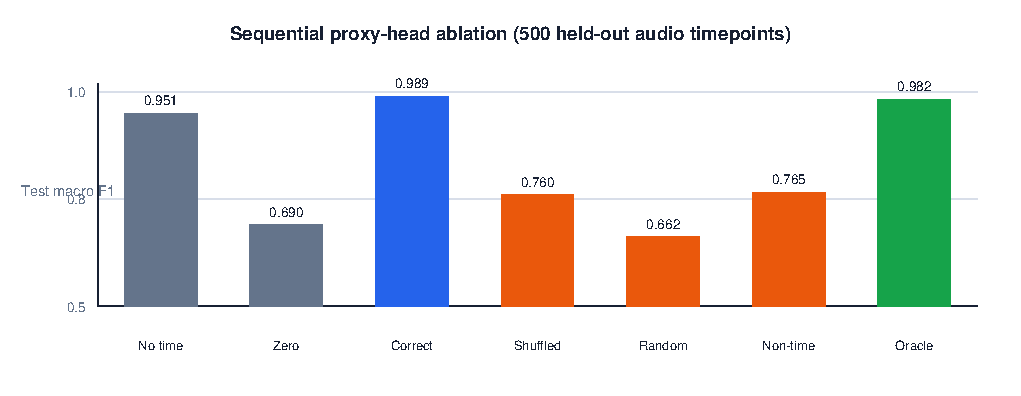
\includegraphics[width=\linewidth]{figures/adapter_ablation.pdf}
\caption{Proxy-head timing ablation at the largest sequential stage. ``Oracle'' is the explicit hidden difference, not privileged access to the label.}
\label{fig:ablation}
\end{figure}

\subsection{Hidden injection alone does not align LM logits}

When the same idea is moved from the auxiliary classifier to the actual generation path, correct-time injection improves macro F1 from 0.297 (no time) to 0.428, but performance remains inadequate. BACKCHANNEL F1 is 0.000, versus 0.569 for WAIT and 0.716 for SUPPORT. Shuffling the adapter still yields 0.396 macro F1, too close to the correct condition to support reliable temporal control.

This result changes the interpretation of the proxy experiment. The residual contains useful information, but the frozen output head has never been trained to map that direction to the desired action tokens. A diagnostic comparison on the same example family gives 0.983 macro F1 for the proxy objective and 0.428 for the base LM objective. Representation reconstruction is therefore insufficient; the decision objective must be aligned.

\subsection{Direct action-token training closes the gap}

Table~\ref{tab:direct} reports the DirectLM scaling experiments. With audio and text prompts, performance rises from 0.663 to 0.983 macro F1 as balanced training grows from 150 to 3,000 points. Oversampling to 6,000 is worse after one epoch and recovers only partially after two, suggesting that balance and coverage matter more than duplicated volume. The strongest audio-only run reaches 0.998 macro F1 and 0.980 exact sequence accuracy.

\begin{table}[t]
\centering
\caption{Direct action-token LoRA results. AT: audio+text; A: audio-only.}
\label{tab:direct}
\small
\begin{tabular}{lrrrr}
\toprule
Train & Input & Acc. & Macro F1 & Exact seq.\\
\midrule
150       & AT & .662 & .663 & .375\\
900       & AT & .897 & .891 & .406\\
3,000     & AT & .984 & .983 & .850\\
6,000 (1 ep.) & AT & .894 & .880 & .400\\
6,000 (2 ep.) & AT & .962 & .960 & .670\\
3,000     & A  & \textbf{.998} & \textbf{.998} & \textbf{.980}\\
\bottomrule
\end{tabular}
\end{table}

The control-plus-response model preserves this behavior: on 500 audio-only test timepoints it reaches 0.998 accuracy and 0.998 macro F1 under correct timing, compared with 0.645 macro F1 without the adapter, 0.616 with shuffled timing, and 0.630 with a random norm-matched residual. Per-class F1 is 0.997 for WAIT, 0.996 for BACKCHANNEL, and 1.000 for SUPPORT. On a 150-item generation subset, 99.3\% begin with the correct control label, all generated continuations match the experiment's simple template-validity rule, and WAIT produces no extra text. The last metric is automated conformance, not a human judgment of response quality.

\begin{figure}[t]
\centering
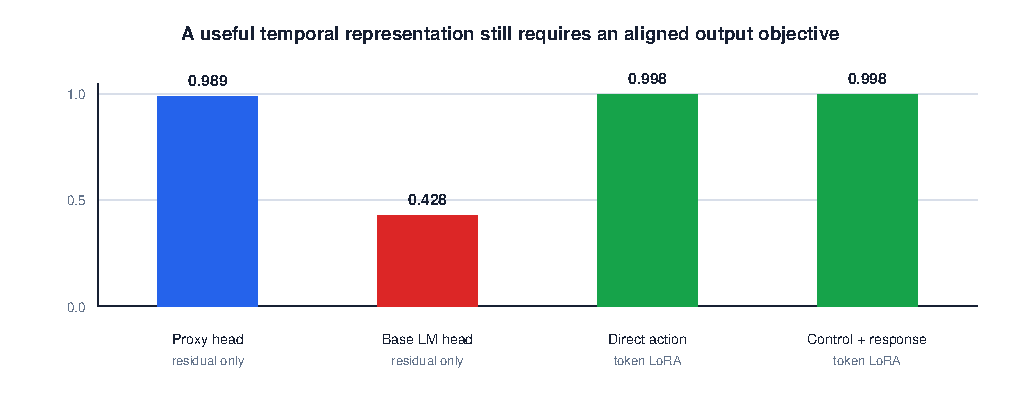
\includegraphics[width=\linewidth]{figures/objective_alignment.pdf}
\caption{Macro F1 across successive objectives. Bars summarize related but not identical splits and therefore illustrate the design progression rather than a controlled model ranking.}
\label{fig:objective}
\end{figure}

\subsection{Local pseudo-realtime latency}

Across 137 action-scoring ticks, mean latency is 295.8 ms, p50 is 270.8 ms, p90 is 300.4 ms, p95 is 309.1 ms, and p99 is 354.0 ms. A cold-start tick takes 3.50 s; 99.3\% of ticks finish within the nominal 500 ms interval. Figure~\ref{fig:latency} excludes the outlying maximum only to keep the central percentiles legible. Short text and speech generation took roughly 1.3--1.5 s in the development snapshots and must remain asynchronous.

\begin{figure}[t]
\centering
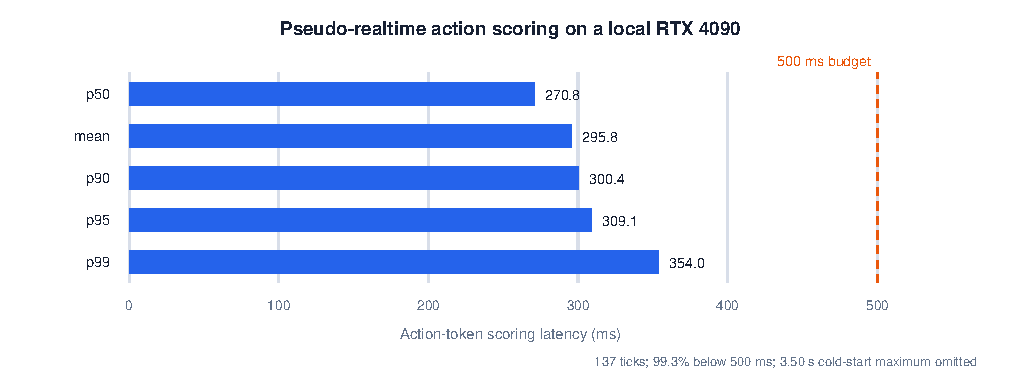
\includegraphics[width=\linewidth]{figures/latency_summary.pdf}
\caption{Local action-scoring latency. The measurement includes only the label-first decision path; generated text and audio are explicitly outside it.}
\label{fig:latency}
\end{figure}

\section{Discussion}

\paragraph{Timing is an interface, not just a latent fact.}
The adapter is best understood as a control interface between a streaming runtime and a pretrained model. The runtime knows how much wall-clock silence has elapsed. Encoding that observation explicitly avoids asking a static audio prefix to represent an ever-changing clock. The strong no-time baseline also shows that audio duration already carries useful evidence; the adapter supplements rather than replaces it.

\paragraph{Proxy success can be misleading.}
An auxiliary classifier can make a representation look solved while the deployed decoder remains unusable. Our largest failure---0.989 proxy macro F1 versus 0.428 under the frozen LM head---is consistent with an objective mismatch. Directly training the three native action-token logits is a small but necessary bridge. This distinction is likely relevant to other activation-steering systems evaluated only with probes.

\paragraph{Separate decision frequency from generation cost.}
A conversational system may need to reconsider turn state several times per second, but it need not synthesize a response at that rate. Short action tokens expose a stable boundary: \code{/W} suppresses work, while \code{/B} and \code{/S} schedule generation. This decomposition also permits debouncing, hysteresis, confidence thresholds, and cancellation to be implemented outside the language model.

\section{Limitations, Ethics, and Artifact Scope}

The reported labels are produced by a deterministic policy over templated English fragments and silence durations. They have no inter-annotator agreement, do not represent culturally variable turn-taking norms, and may reward learning the generator's structure. Qwen3-TTS audio and appended digital silence are cleaner than natural microphones, rooms, cross-talk, and network jitter. The local recording check is too small for accuracy claims. No user study, multilingual evaluation, public conversational benchmark, or human response-quality rating was conducted.

Several comparisons use related but non-identical splits or training objectives; Figure~\ref{fig:objective} is consequently not a strict leaderboard. Hyperparameters were selected during iterative research, so the test numbers should not be treated as untouched confirmatory evaluation. The latency result is specific to one RTX 4090 environment, includes a substantial cold start, and excludes asynchronous generation. A production system must additionally address barge-in, VAD errors, ASR revisions, concurrency, safety, and graceful degradation.

No private conversation logs are published. The public repository contains source snapshots, aggregate results, and documentation, but excludes recordings, generated dataset rows, model weights, caches, and private evaluation material while provenance is reviewed. Code is MIT-licensed; third-party model and data terms remain controlling. In particular, the Qwen2.5-Omni-3B checkpoint used by these experiments is distributed under its own research license with non-commercial restrictions. This source release does not relicense or redistribute it.

\section{Reproducibility}

The source release is available at
\begin{center}
\url{https://github.com/onigirikiller/time-adapter-research}.
\end{center}
The repository maps each claim to executable snapshots: dataset generation, sequential proxy evaluation, generation-hook diagnosis, DirectLM LoRA training, control-plus-response training, and pseudo-realtime scoring. Aggregate figure values are encoded in a small plotting script so the paper can be rebuilt without private artifacts. Reproducing model results requires downloading the applicable upstream checkpoints, accepting their licenses, regenerating the data, and using a compatible PyTorch/CUDA environment. Seeds are recorded in the scripts, but GPU kernels and generation stacks may still be nondeterministic.

\section{Conclusion}

We presented a compact Time Adapter for injecting externally measured streaming time into an audio-language model and a label-first runtime for deciding whether to wait, backchannel, or respond. On generated sequential data, the adapter supports high proxy accuracy, but the frozen LM head exposes a decisive objective mismatch. Training three single-token action logits with LoRA closes that gap, while separating action scoring from response generation meets a 500 ms local tick budget after warm-up. The central claim is therefore modest: explicit temporal residuals are useful when the deployed output objective is trained to consume them. Natural-dialogue annotation, multilingual evaluation, human judgments, and broader hardware tests are required before production conclusions.

\section*{Acknowledgments}

The author conducted this research independently and thanks the maintainers of the open-source model and software ecosystems used in the experiments.

\bibliographystyle{plain}
\bibliography{references}

\appendix
\section{Experiment Configuration}

\begin{center}
\captionof{table}{Main configuration recorded by the released scripts.}
\small
\begin{tabular}{ll}
\toprule
Component & Setting\\
\midrule
Audio LM & Qwen2.5-Omni-3B\\
TTS & Qwen3-TTS-0.6B CustomVoice\\
Timepoints (s) & 0, .25, .5, .75, 1, 1.5, 2, 3, 4, 6\\
Main injection & layer 3, $\alpha=4$, all tokens\\
Action tokens & \code{/W}, \code{/B}, \code{/S}\\
LoRA & rank 8, scale 16, dropout .05\\
LoRA targets & q/k/v/o, gate/up/down projections\\
Control response & 2 epochs, LR $10^{-4}$\\
Control-token weight & 4.0\\
Tick interval & 500 ms\\
\bottomrule
\end{tabular}
\end{center}

\noindent\begin{minipage}{\linewidth}
\section{Full Proxy Ablation}

\begin{center}
\captionof{table}{Largest-stage proxy-head test results (500 timepoints).}
\small
\begin{tabular}{lrrr}
\toprule
Condition & Acc. & Macro F1 & Exact seq.\\
\midrule
No time hidden & .956 & .951 & .700\\
Audio only & .498 & .399 & .280\\
Zero vector & .752 & .690 & .380\\
Correct adapter & .990 & .989 & .920\\
Shuffled adapter & .790 & .760 & .380\\
Random norm-matched & .718 & .662 & .360\\
Non-time numeric & .794 & .765 & .440\\
Oracle explicit delta & .984 & .982 & .860\\
\bottomrule
\end{tabular}
\end{center}
\end{minipage}

\section{Claim Boundaries}

The paper uses ``time'' in three distinct senses. First, the runtime observes wall-clock features such as elapsed silence. Second, an explicit textual cue is used only to define a hidden-difference training target. Third, audio waveforms are physically extended by silence, so the no-time baseline can still observe prefix duration. The experiments do not show that a model can recover an unobserved external clock, nor that the three programmatic actions are a universal ontology of conversational behavior.

\end{document}
